% -*- program: xelatex -*-
\documentclass[11pt, compress]{beamer} 

%\usefonttheme[onlymath]{serif}
\DeclareFontEncoding{T1}
\fontencoding{T1}
\usepackage[T2A]{fontenc}
\usepackage[utf8]{inputenc}
\usepackage[russian]{babel}
\usepackage{listings}
\usepackage{amsmath,amssymb,amsthm} 
\hypersetup{unicode=true}
\usepackage{color}
\definecolor{mygreen}{RGB}{28,172,0} % color values Red, Green, Blue
\definecolor{mylilas}{RGB}{170,55,241}
\definecolor{codecolor}{RGB}{0,120,0}
\newcommand{\matcode}[1]{ \textcolor{codecolor}{\texttt{#1}}}
\usepackage{graphics,graphicx}
\usepackage{verbatim}
\usepackage{fancyvrb}
\usepackage{booktabs}
%\usepackage{media9}

 
\newcommand{\cleartitlepage}[1]{\begin{frame}[plain]\begin{center}\textsc{#1}\end{center}\end{frame}}
\usetheme{m} 

\usepackage{tikz}
\usetikzlibrary{positioning} 
\tikzset{cbutton/.style={rectangle,minimum width=10mm,thick,draw=red!50!black!50,
top color=white,bottom color=red!50!black!30}}
\tikzset{mbutton/.style={rectangle,minimum width=10mm,thick,draw=black!20,
top color=white,bottom color=black!30}}

\lstset{language=Matlab,    
    keepspaces=true,
    extendedchars=true,
    basicstyle={\footnotesize  \color{black}},
    breaklines=true,
    morekeywords={matlab2tikz},
    keywordstyle=\color{blue},
    morekeywords=[2]{1}, keywordstyle=[2]{\color{codecolor}},
    identifierstyle={ \bf \color{black} },
    stringstyle=\color{mylilas},
    commentstyle=\color{mygreen},%
    showstringspaces=false,
    numbers=left,%
    numberstyle={\tiny \color{black}},
    numbersep=7pt, 
    emph=[1]{case,switch,otherwise},emphstyle=[1]\color{blue}, 
    frame=single,    
    %lineskip=-1.0pt,
    %emph=[2]{word1,word2}, emphstyle=[2]{style},    
}

\title{Численные методы}
\subtitle{Основы MATLAB}
\author{Юдинцев В. В.}
\small
\institute[СГАУ]
{
Кафедра теоретической механики \\
Самарский государственный аэрокосмический университет \\ им. академика С.~П.~Королёва \\
(национальный исследовательский университет) \\
\vfill
{http://yudintsev.info}
}

\begin{document}

{
\usebackgroundtemplate{
\includegraphics[width=\paperwidth,height=\paperheight]{../matlablogo.png}}
\maketitle
}

\frame{
\frametitle{Содержание}
\tableofcontents
}
%
%
\section{Интерполирование табличных данных}
%
%
\frame{
\frametitle{Полиномиальная интерполяция}
\begin{itemize}
 \item Известны значения некоторой функции $y(x)$ в точках $x_0, x_1, x_2, \ldots, x_n$:
$$
  y_0, y_1, y_2, \ldots, y_n.
$$  
 \item Необходимо построить интерполирующий многочлен $L_{n}(x)$, совпадающий с значениями табличной функции в точках $x_0, x_1, x_2, \ldots, x_n$ и приближающий функцию $y(x)$ на интервале $[x_0,x_n]$.
\end{itemize}
Интерполирующий многочлен в форме Лагранжа:
$$
L_{n}=\sum_{i=0}^{n}y_{i}\dfrac{(x-x_{0})(x-x_{1})...(x-x_{i-1})(x-x_{i+1})...(x-x_{n})}{(x_{i}-x_{0})(x_{i}-x_{1})...(x_{i}-x_{i-1})(x_{i}-x_{i+1})...(x_{i}-x_{n})}
$$
}

\frame[containsverbatim]
{
\frametitle{Полиномиальная интерполяция: функция polyfit}
Исходные данные
\begin{lstlisting}
x = [0.1 0.2 0.3 0.4];
y = [0.2 0.6 0.5 0.3];
\end{lstlisting}
Вычисление коэффициентов интерполирующего многочлена $\tilde{y} = p_n x^{n} + p_{n-1} x^{n-1} + \ldots + p_0 $ для $n = 3$ 
\begin{lstlisting}[firstnumber=last]
p = polyfit(x,y,3)
ans =
    66.6667  -65.0000   18.8333   -1.1000
\end{lstlisting}
Первый элемент -- $p_n$, последний -- $p_0$.
}

\frame[containsverbatim]
{
\frametitle{Вычисление значения интерполирующей функции}
Значения многочлена в точке $x=0.15$:
\begin{lstlisting}[firstnumber=last]
>> polyval(p,0.15)
ans = 
      0.48750
\end{lstlisting}      
}

\frame[containsverbatim]
{
\frametitle{Полиномиальная интерполяция}
\begin{center}
 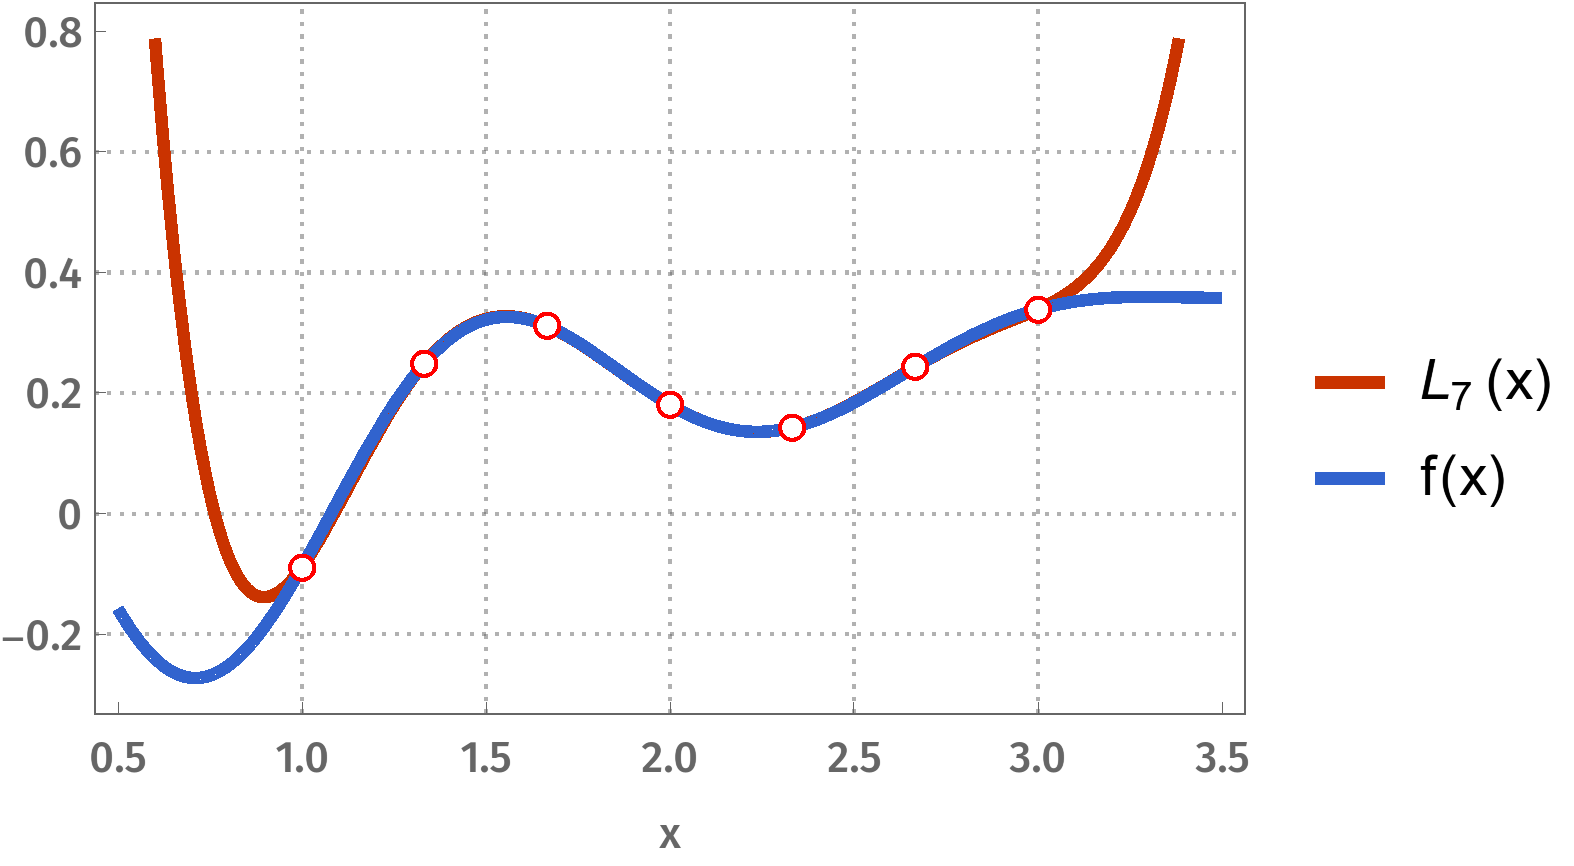
\includegraphics[width=0.85\linewidth]{./PolyInterpolation.png}
 % PolyInterpolation.png: 1573x847 pixel, 300dpi, 13.32x7.17 cm, bb=0 0 378 203
\end{center}
}

\frame[containsverbatim]
{
\frametitle{Полиномиальная интерполяция}
\begin{center}
 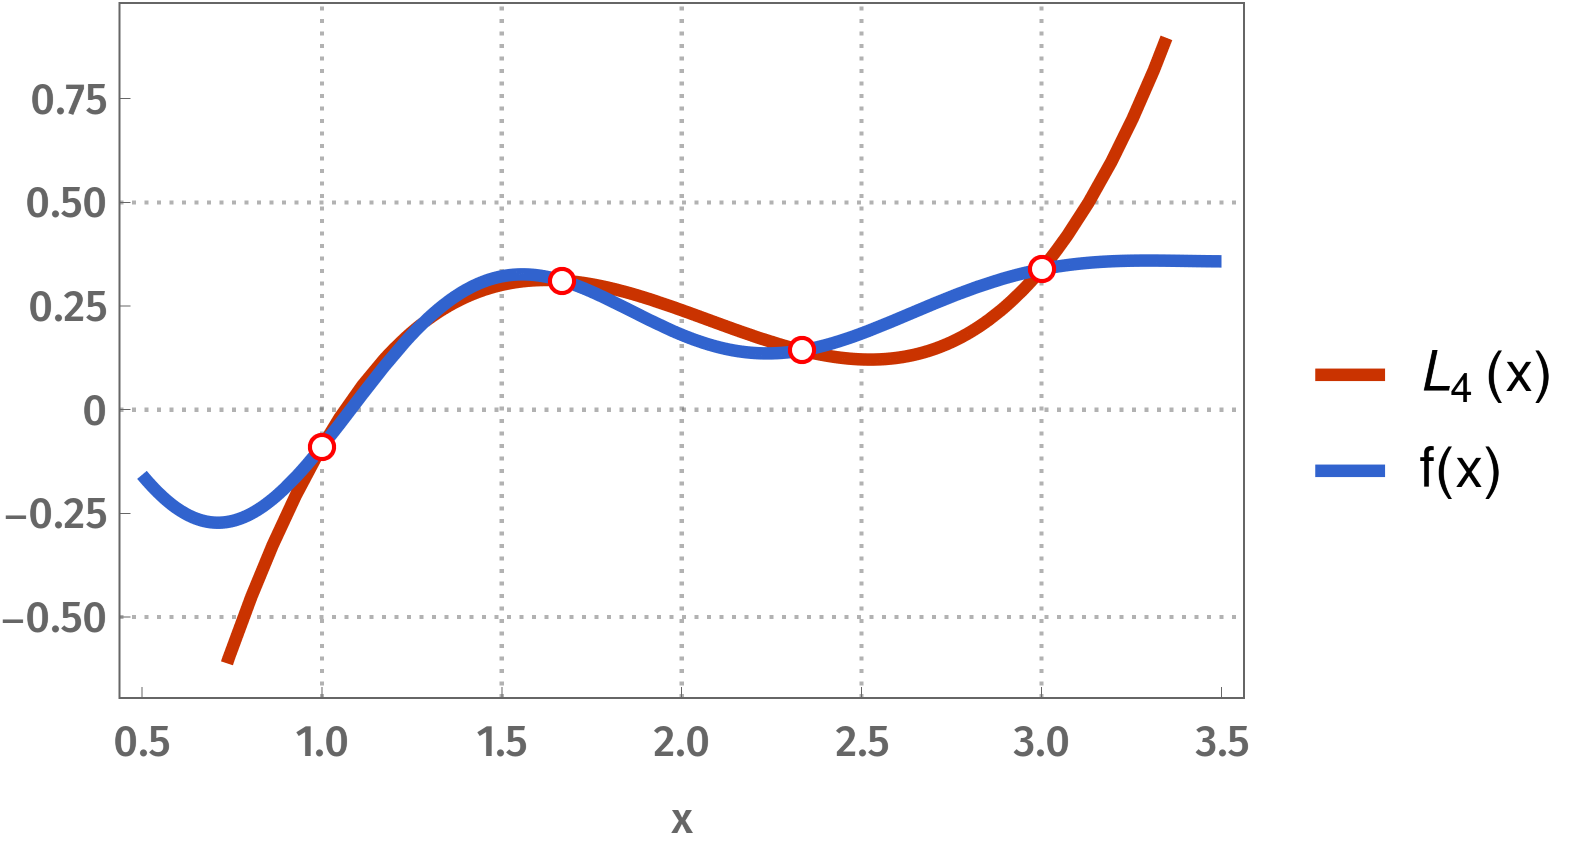
\includegraphics[width=0.85\linewidth]{./PolyInterpolation2.png}
 % PolyInterpolation.png: 1573x847 pixel, 300dpi, 13.32x7.17 cm, bb=0 0 378 203
\end{center}
}

\frame[containsverbatim]
{
\frametitle{Полиномиальная интерполяция}
\begin{itemize}
 \item Полиномиальная интерполяция используется локально. 
\begin{center}
 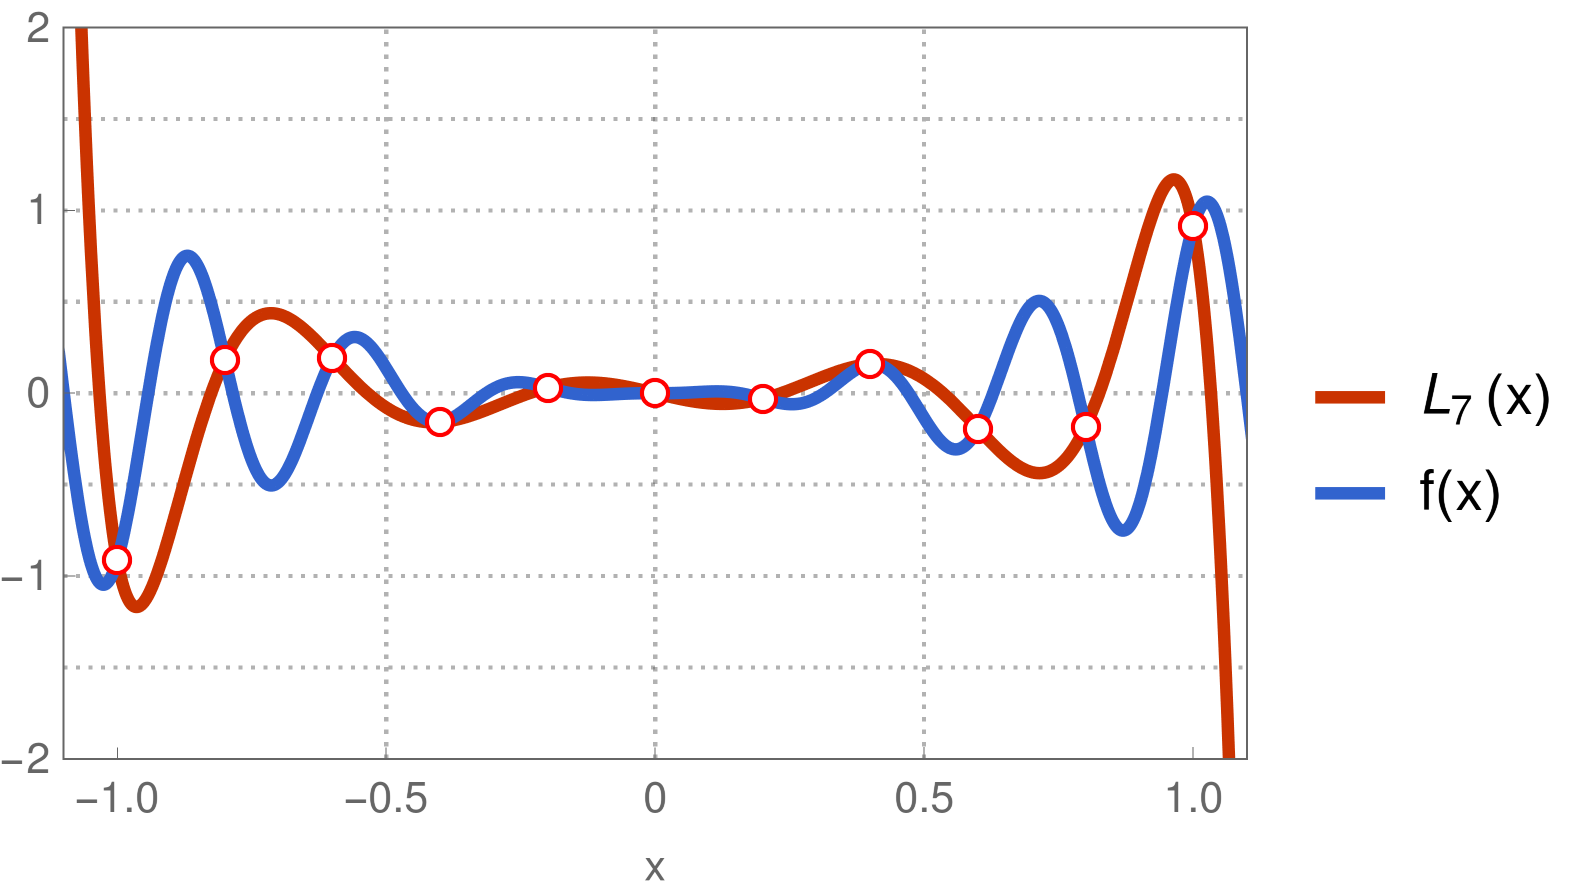
\includegraphics[width=0.7\linewidth]{./PolyInterpolationBad.png}
 % PolyInterpolation.png: 1573x847 pixel, 300dpi, 13.32x7.17 cm, bb=0 0 378 203
\end{center}
 \item Для глобальной интерполяции используется сплайн-интерполяция -- глобальная "`кусочно-полиномиальная"' интерполяция. 
\end{itemize}
}

\frame[containsverbatim]
{
\frametitle{Построение графика}
\begin{lstlisting}[firstnumber=last]
>> fplot(@(x) polyval(p,x),[0.1 0.4]);
>> grid on;
>> xlabel('x');ylabel('y');
>> print('-dpng', '-r600', 'function.png');
\end{lstlisting}      
\begin{center}
 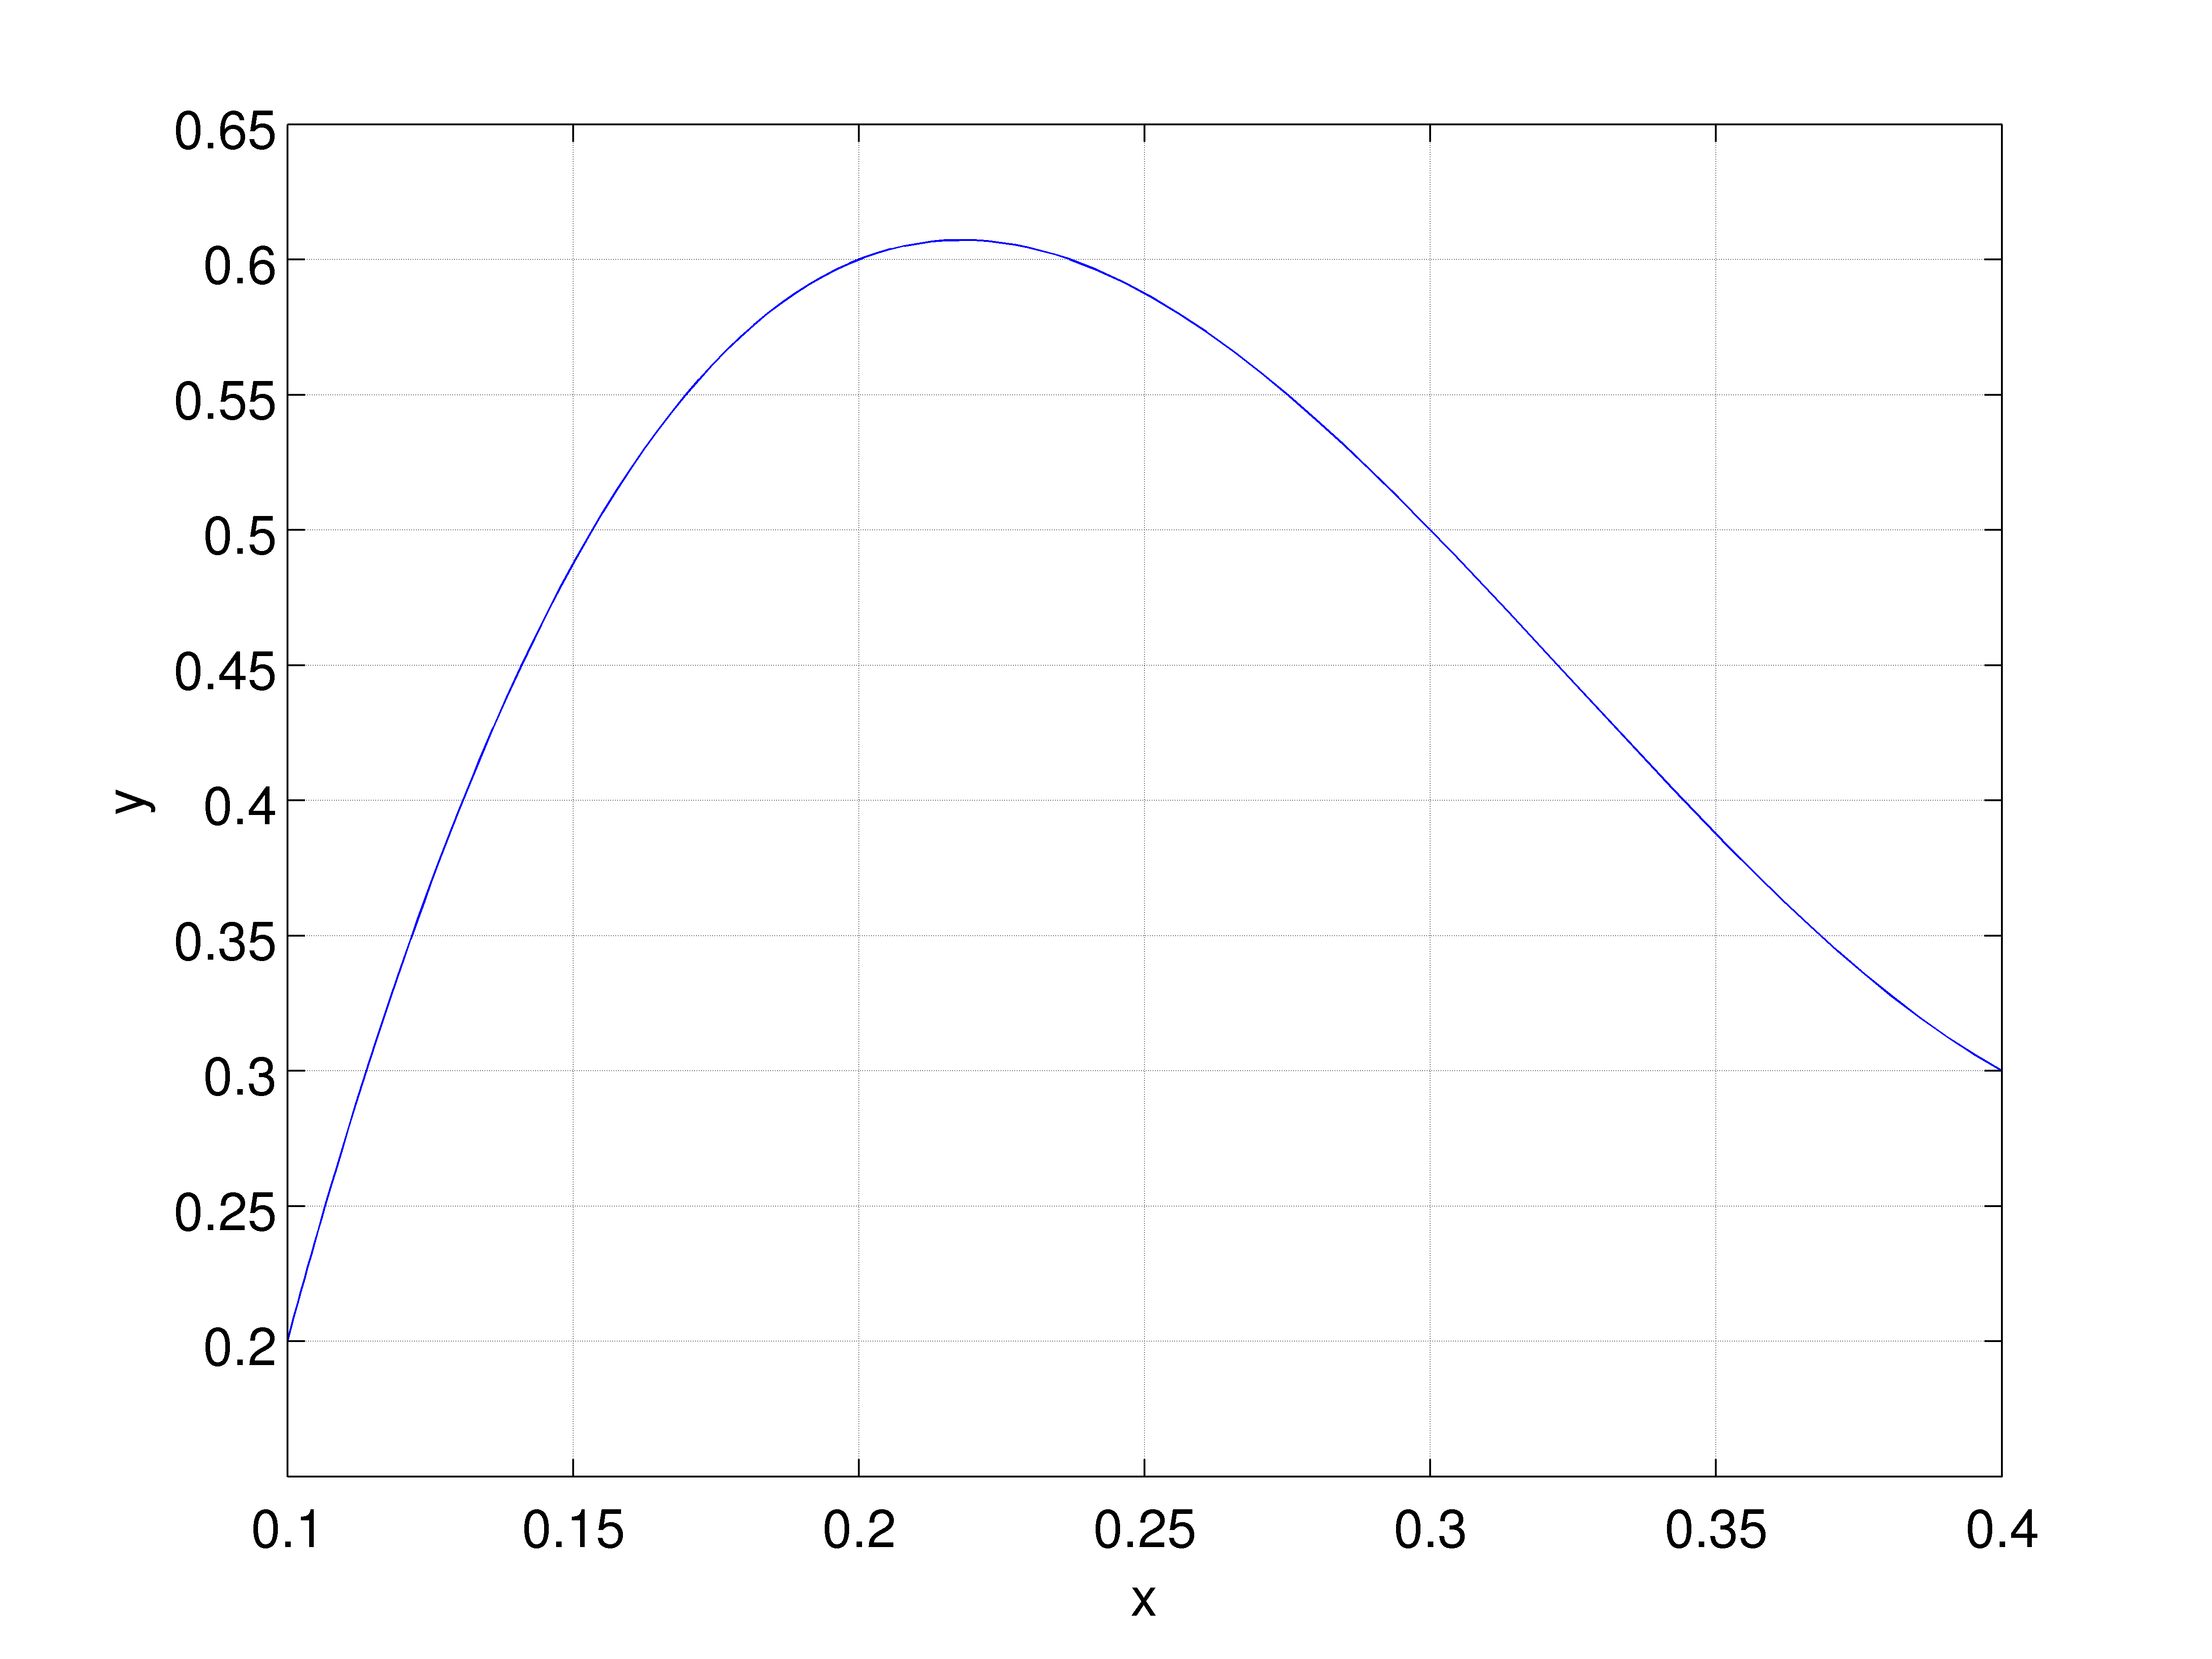
\includegraphics[width=0.6\linewidth]{./function.png}
\end{center}
}

\frame[containsverbatim]
{
\frametitle{Сплайн-интерполяция}
Для числа или вектора/матрицы \matcode{xp}:
линейная интерполяция 
\begin{lstlisting}
yp = interp1(x,y,xp)
\end{lstlisting}
поиск ближайшего табличного значения 
\begin{lstlisting}
yp = interp1(x,y,xp,'nearest')
\end{lstlisting}
сплайн-интерполяция (полином 3 степени) 
\begin{lstlisting}
yp = interp1(x,y,xp,'spline')
\end{lstlisting}
}
%
%
\section{Численное дифференцирование}
%
%
\frame[containsverbatim]
{
\frametitle{Конечные разности}
Задана таблица значений $x_0,x_1,x_2,\ldots,x_n$:
\begin{lstlisting}
>> x = [0.1 0.21 0.32 0.41];
\end{lstlisting}
Конечные разности 1-го порядка 
$$
\Delta x_k = x_{k+1}-x_k, \; k=0,\ldots,n-1
$$ 
\begin{lstlisting}
>> dx = diff(x)
ans =
      0.110000   0.110000   0.090000
\end{lstlisting}
Конечная разности 2-го порядка 
\begin{lstlisting}
>> dx = diff(x,2)
ans =
     2.7756e-17  -2.0000e-02
\end{lstlisting}
}
%
%
\section{Численное интегрирование}
%
%
\frame[containsverbatim]
{
\frametitle{Метод трапеций}
\begin{columns}
\column{0.5\linewidth}
\begin{figure}[htbp]
	\centering
	
\includegraphics[width=1\textwidth]{Simpson.pdf}	
\end{figure}
\column{0.5\linewidth}
Табличная функция:
\begin{lstlisting}
>> x = [0.1 0.21 0.32 0.41];
>> y = sin(x)+x;
\end{lstlisting} 
Вычисление интеграла:
\begin{lstlisting}
>> trapz(x,y)
ans = 
    0.1569
\end{lstlisting} 
\end{columns}
$$
\int_a^b y(x) dx \approx \frac{1}{2} \sum_{i=1}^n (x_{n+1}-x_n) (y_n + y_{n+1})
$$
}

\frame[containsverbatim]
{
\frametitle{Метод Симпсона}
Интегрирование методом Симпсона
\begin{lstlisting}
integral = quad(@function,a,b,eps);
\end{lstlisting}
\matcode{a,b} -- пределы интегрирования 

\matcode{eps} -- точность (по умолчанию $10^{-6}$)

\matcode{@function} -- ссылка на функцию или строка-выражение, например,\matcode{'sin(x)+x'}.
}
%
%
%
\section{Интегрирование ОДУ}
%
%
%
\begin{frame}{Структура}
$$
\left\{
\begin{aligned}
& \frac{d q_1}{dt} = f_1(t,q_1,q_2,\ldots,q_n),  \\
& \frac{d q_2}{dt} = f_2(t,q_1,q_2,\ldots,q_n),  \\
& \ldots \\
& \frac{d q_n}{dt} = f_n(t,q_1,q_2,\ldots,q_n).  
\end{aligned}
\right. 
\quad \Rightarrow \quad
\frac{d \boldsymbol q}{dt} = \boldsymbol f(t,\boldsymbol q)
$$
где 
\begin{itemize}
	\item $\boldsymbol q = (q_1,q_2,\ldots,q_n)$ -- вектор состояния;
	\item $\boldsymbol f(t,\boldsymbol q)$ -- вектор-функция правых частей.
\end{itemize}
\end{frame}

\begin{frame}{Структура}
\begin{itemize}
	\item Приведение к системе дифференциальных уравнений первого порядка.
	\item Файл-функция правой части $\boldsymbol f(t,\boldsymbol q)$.
	\item Файл-скрипт запуска процесса интегрирвования ДУ.
\end{itemize}
\end{frame}

\section{Пример: задача баллистики}

\begin{frame}{Задача баллистики}
	\begin{figure}[htbp]
		\centering
		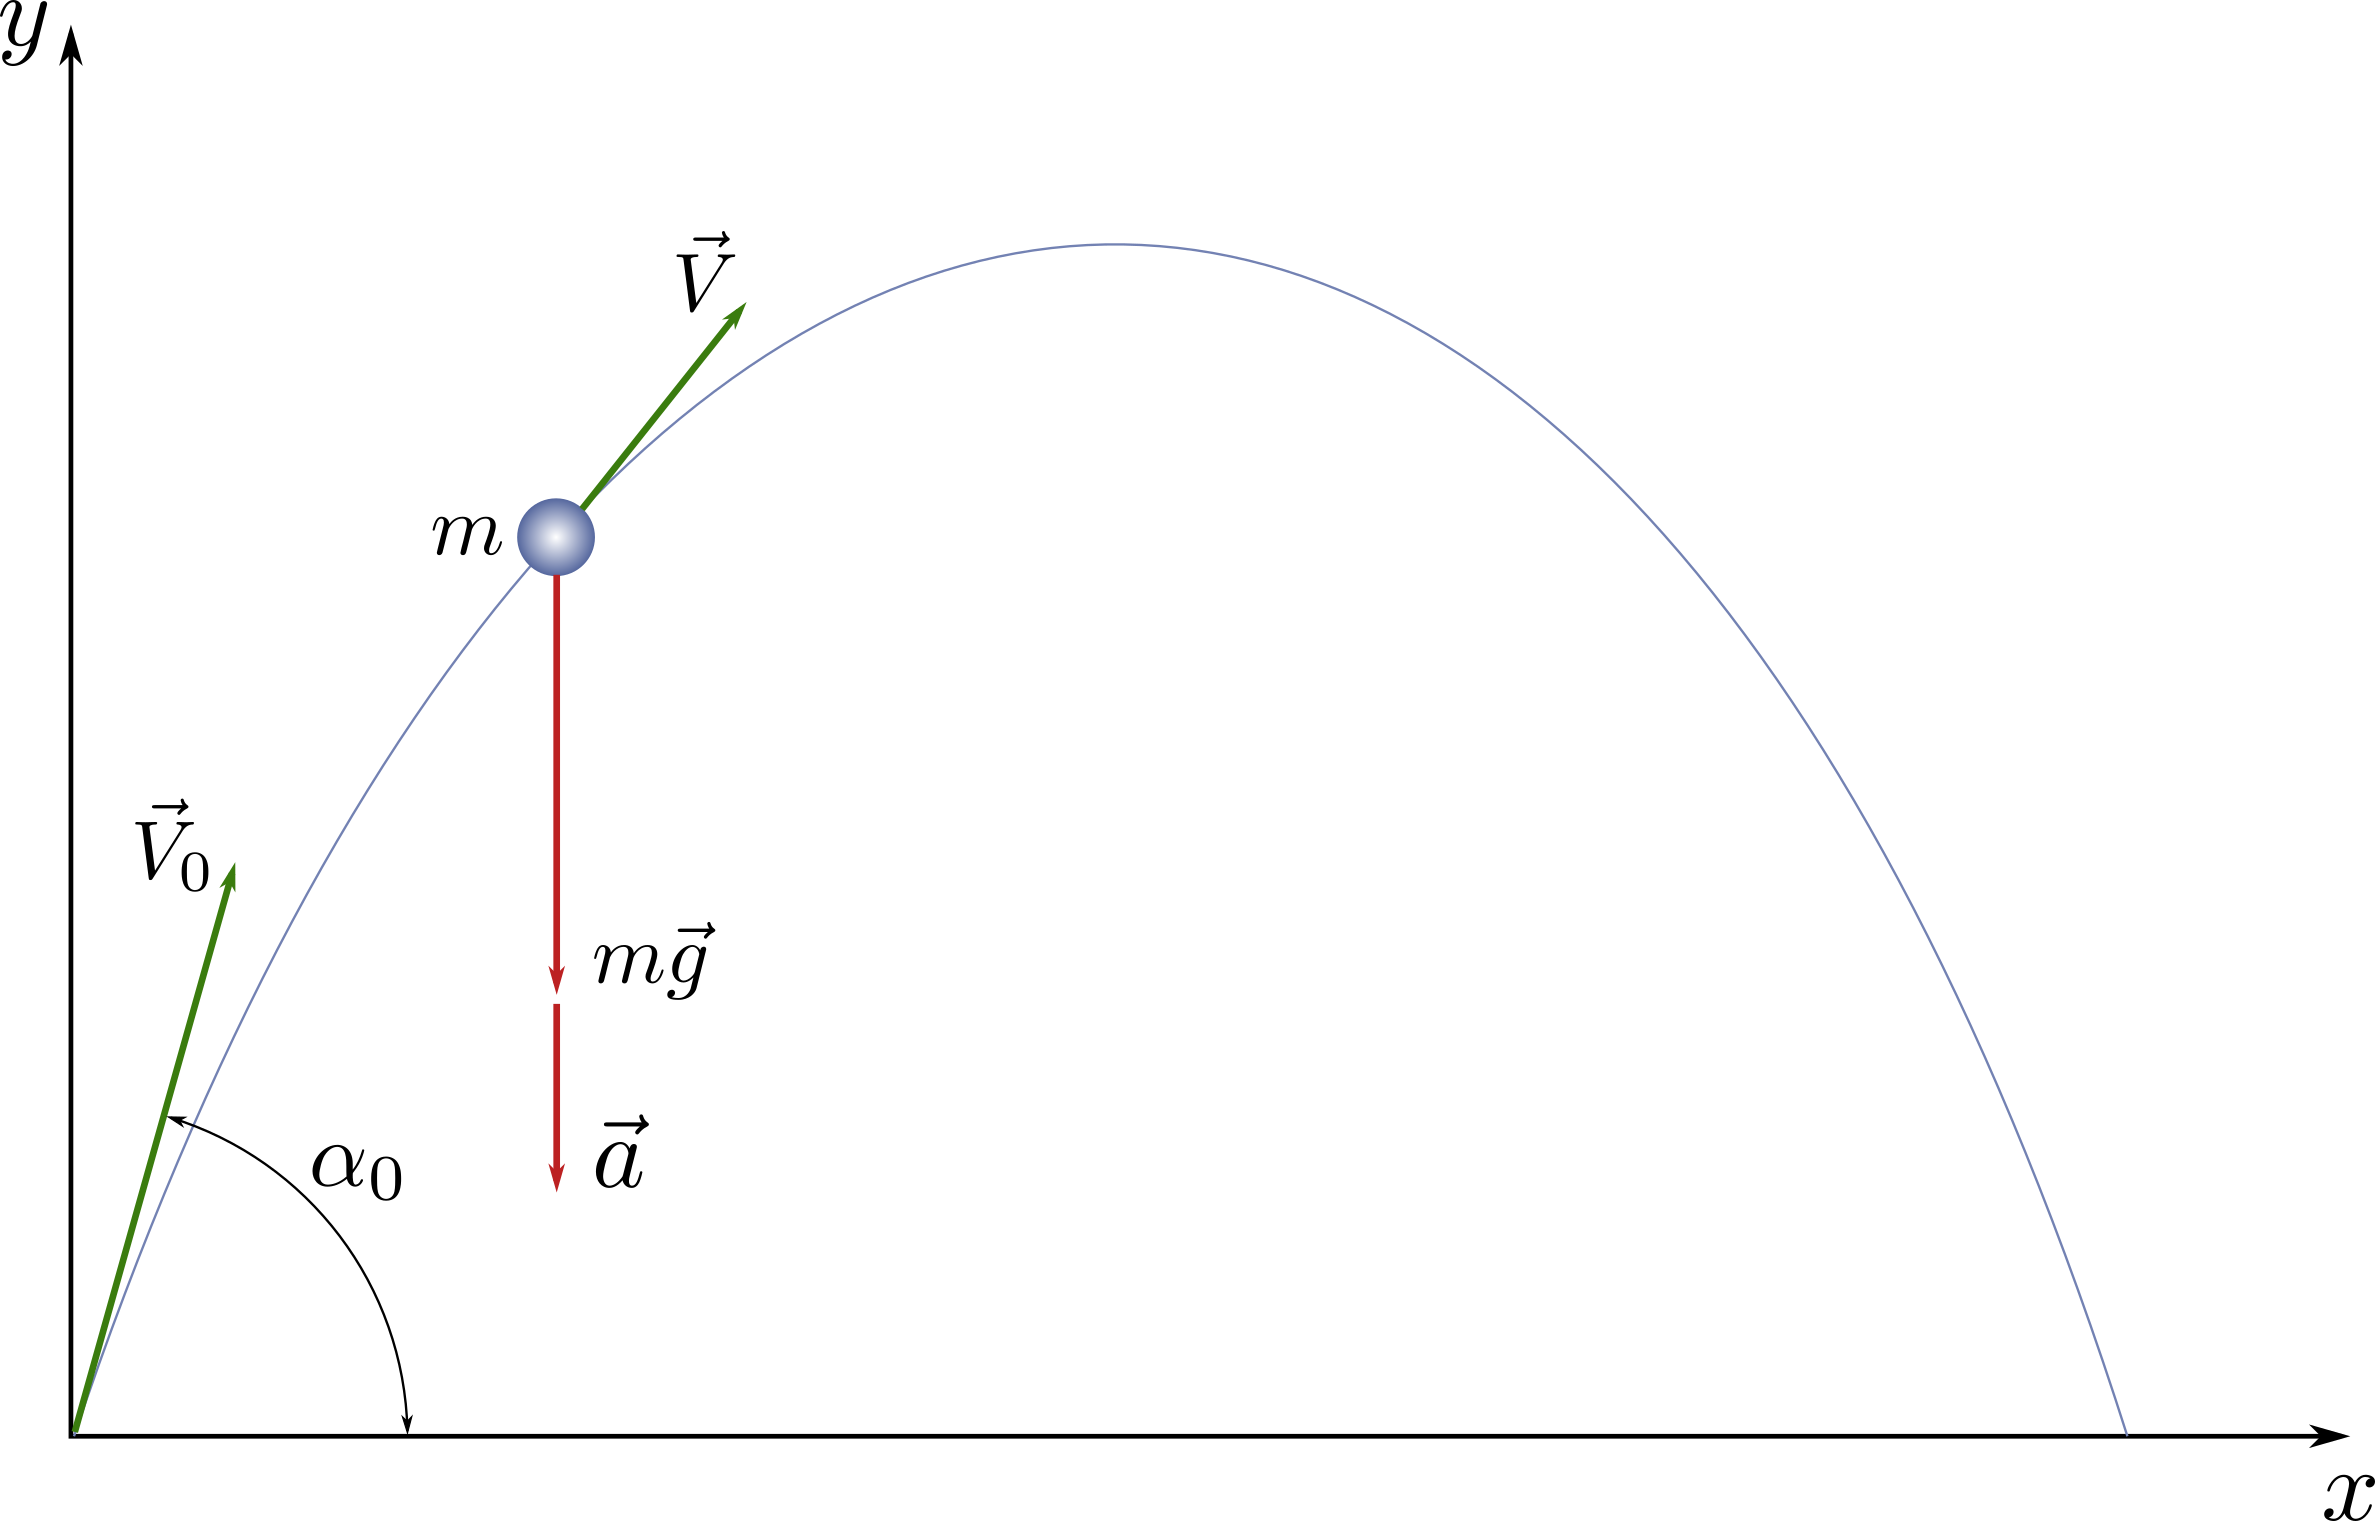
\includegraphics[width=1\textwidth]{Fall1.png}
	\end{figure}
\end{frame}

\begin{frame}{Уравнения движения}
\begin{columns}
\column{0.4\linewidth}
	\begin{figure}[htbp]
		\centering
		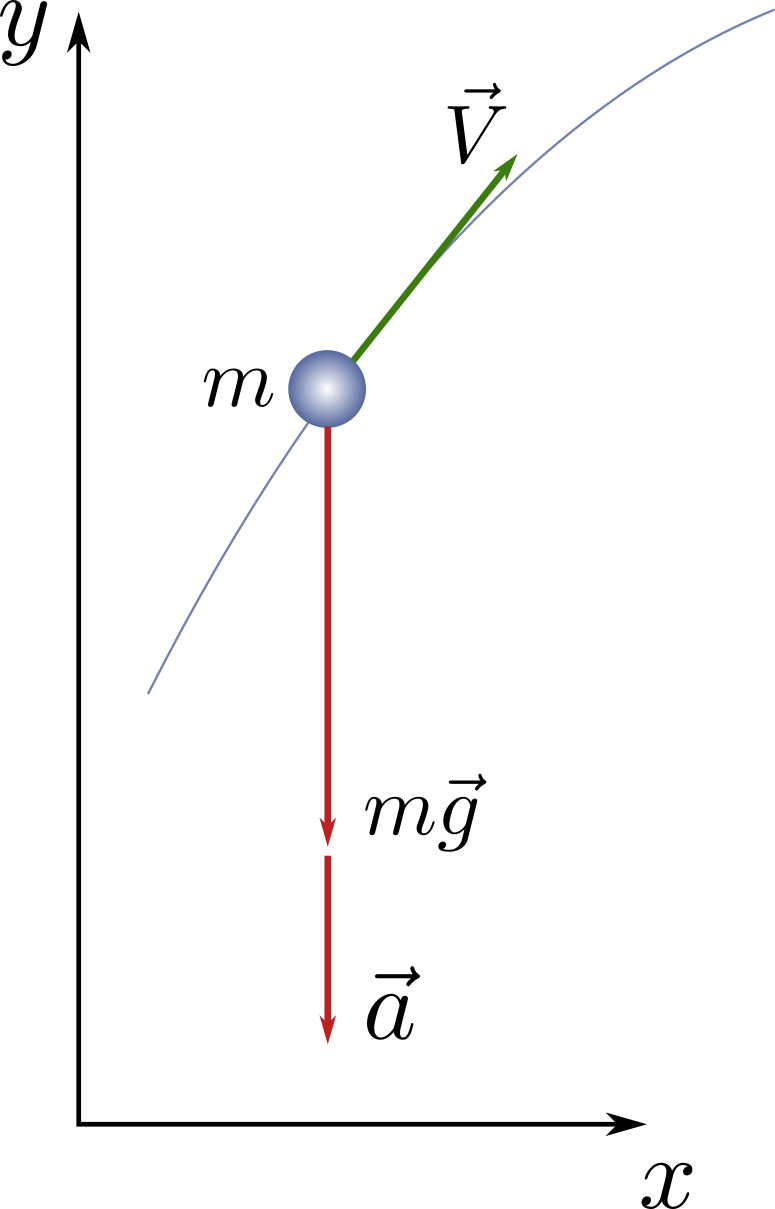
\includegraphics[width=1\textwidth]{Fall2.png}
	\end{figure}
\column{0.6\linewidth}
Векторное уравнение
$$
	m \vec a = \vec F_g = m \vec g.
$$	
Проекции векторного уравнения на оси координат:
$$
\begin{aligned}
	& m a_x = m \frac{d^2x}{dt^2} = 0, \\
	& m a_y = m \frac{d^2y}{dt^2} = - m g.
\end{aligned}
$$	
\end{columns}
\end{frame}



\frame
{
\frametitle{Дифференциальные уравнения движения}
Приведение к системе дифференциальных уравнений первого порядка.
$$
\left\{
\begin{aligned}
& m \frac{d^{\,2} x}{dt^2} = 0,  \\
& m \frac{d^{\,2} y}{dt^2} = - m g.
\end{aligned}
\right. 
\quad \Rightarrow \quad
   \left\{
   \begin{aligned}
   & \frac{dx}{dt} = V_x,  \\   
   & \frac{dV_x}{dt} = 0, \\
   & \frac{dy}{dt} = V_y,  \\
   & \frac{dV_y}{dt} = - g.
   \end{aligned}
   \right.
   \quad \Rightarrow \quad
   \frac{d \boldsymbol q}{dt} = \boldsymbol f(\boldsymbol q, t)
$$
где
$$
	\boldsymbol q=(x,V_x,y,V_y), \quad \boldsymbol f(\boldsymbol q, t) = (V_x,0,V_y,-g)
$$
}


\frame[containsverbatim]
{
\frametitle{ODE файл -- файл-функция правых частей}
Файл в котором вычисляется правая часть дифференциального уравнения или системы уравнений:
$$
  \mathbf q \Rightarrow \boxed{ \dot{\mathbf q} = \mathbf f(\mathbf q,t) }  \Rightarrow  \dot {\mathbf q}
$$
где $\mathbf q$ -- вектор зависимых переменных, $t$ -- время.

Файл-функция \matcode{dqdt.m}
\begin{lstlisting}
function dq = dqdt(t,q)
	g = 9.81;
	m = 1.00;
	x=q(1); Vx=q(2); y=q(3); Vy=q(4);
	dq = [Vx, 0, Vy, -g];
\end{lstlisting}
}

\frame[containsverbatim]
{
\frametitle{Интегрирование}
\begin{columns}
\column{0.25\linewidth}
	\begin{figure}[htbp]
		\centering
		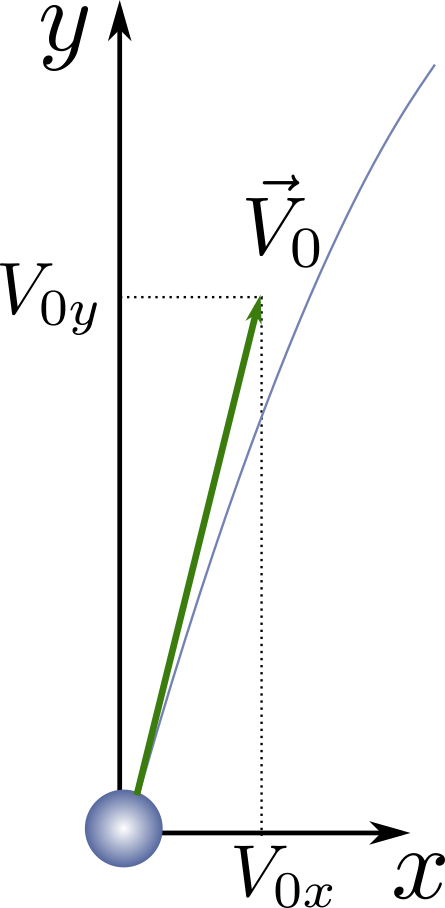
\includegraphics[width=1\textwidth]{Fall3.png}
	\end{figure}
\column{0.75\linewidth}
\begin{lstlisting}
% Начальные условия
V0 = 10;
a  = pi/4;
q0 = [0, V0*cos(a), 0, V0*sin(a)];
% Интервал интегрирования
tspan = [0 5];
[t, q] = ode45(@dqdt, tspan, q0);
\end{lstlisting}
\end{columns}
}

\frame[containsverbatim]
{
\frametitle{Методы интегрирования}
\begin{table}[h]
\center
\begin{tabular}{@{}lp{0.8\linewidth}@{}}
\toprule
Интегратор & Описание \\
 \cmidrule{1-2}
 \matcode{ode45} & Метод Рунге-Кутты 4 и 5 порядков с автоматическим выбором шага  \\
 \matcode{ode23} & Метод Рунге-Кутты 2 и 3 порядков с автоматическим выбором шага  \\
 \matcode{ode113} & Многошаговый метод Адамса: метод с предсказанием и коррекцией \\
 \matcode{ode15s} & Многошаговый метод для интегрирования жестких систем \\
 \matcode{ode23s} & Одношаговый метод Розенброка второго порядка для жестких систем \\
\bottomrule
\end{tabular}
\end{table}
}

\frame[containsverbatim]
{
\frametitle{Результаты интегрирования}
\begin{lstlisting}
[t, q] = ode45(@dqdt, tspan, q0);
\end{lstlisting}
\vspace{16pt}
\begin{columns}
\column{.5\textwidth}
  \matcode{t} -- столбец независимой переменной (время) \\
  $$ t = \begin{bmatrix} t_0 \\ t_1 \\ \ldots \\ t_k \end{bmatrix}$$
\column{.5\textwidth}
  \matcode{q} -- матрица зависимых переменных
  $$ q = \begin{bmatrix} x_0 & V_{x0} & y_0 & V_{y0} \\  x_1 & V_{x1} & y_1 & V_{y1} \\ \ldots \\ x_k & V_{xk} & y_k & V_{yk} \end{bmatrix}$$
\end{columns}
}

\section{Управление процессом интегрирования}

\frame[containsverbatim]
{
\frametitle{Управление процессом интегрирования}
Расширенная версия запуска интегрирования д.у.:
\begin{lstlisting}
[t, q] = ode45( @dqdt, tspan, q0, options);
\end{lstlisting}
\vspace{16pt}
До запуска интегрирования заполняется специальная структура  \matcode{options} при помощи функции \matcode{odeset}: 
\begin{lstlisting}
options = odeset('Парам. 1', Значение, 'Парам. 2', ...);
[t, q] = ode45( @dqdt, tspan, q0, options);
\end{lstlisting}
}

\frame[containsverbatim]
{
\frametitle{Точность решения}
\begin{itemize}
  \item \matcode{'RelTol'}: относительная погрешность. \textbf{Число} - значение погрешности для всех переменных, или \textbf{вектор}, задающий погрешность для каждой переменной (по умолчанию $10^{-3}$)
  \item \matcode{'AbsTol'}: абсолютная погрешность. Число или вектор (по умолчанию $10^{-6}$)
\end{itemize}
\vfill
\begin{lstlisting}
options = odeset('RelTol',1e-4,'AbsTol',1e-8);
[t, q] = ode45( @dqdt, tspan , q0, options );
\end{lstlisting}
}

\frame[containsverbatim]
{
\frametitle{Параметры интегрирования}
\begin{itemize} 
  \item \matcode{'InitialStep'}: начальный шаг интегрирования;
  \item \matcode{'Mass'}: матрица коэффициентов $\mathbf M$ в дифференциальных уравнениях, записанных в виде 
$$
\mathbf M(\mathbf q,t) \dot{\mathbf q} = \mathbf f(t,\mathbf q). 
$$
Имя переменной, если матрица масс постоянная, или ссылка на m-файл. Для всех интеграторов кроме \matcode{ode15s, ode23t} матрица масс должна быть невырожденная;
 \item \matcode{'MassSingular'}: может ли матрица масс быть вырожденной. Возможные значения: \matcode{'yes'}, \matcode{'no'}, \matcode{'maybe'} (по умолчанию \matcode{'maybe'}).
\end{itemize}
}

\frame[containsverbatim]
{
\frametitle{События: параметр 'Events'}
Для остановки процесса интегрирования при выполении некоторого условия используется функция событий, которая передаётся интегратору:
\begin{lstlisting}
options = odeset('Events',@events);
\end{lstlisting}
\begin{lstlisting}[firstnumber=last]
V0 = 1; 
a  = pi/4;
q01 = [0,V0*cos(a),0,V0*sin(a)];
[t1,q1] = ode45(@dqdt,[0 20],q01);
\end{lstlisting}
}

\begin{frame}[fragile]{Пример файл-функции событий events.m}
$$
\boldsymbol q=(x,V_x,y,V_y)^T
$$
\begin{lstlisting}
function [ value, isterminal, direction ] = events(t, q)
 % Следим за изменением переменной y
 value = q(3); 
 % Остановить процесс, 
 isterminal= 1;
 % если q(3) станет равна нулю и будет убывать
 direction =-1;
\end{lstlisting}
Файл-функция для остановки процесса интегрирования (\alert{isterminal=1}) при пересечении нуля функцией $y(t)$ (\alert{value = q(3)}) при её убывании (\alert{direction = -1}).
\end{frame}

\frame[containsverbatim]
{
\frametitle{Падение шарика на упругую поверхность}
\begin{lstlisting}
options = odeset('Events',@events);
v0 = 1; 
q01 = [0,v0*cos(pi/4),0,v0*sin(pi/4)];
[t1,q1] = ode45(@dqdt,[0 20],q01);
\end{lstlisting}
\begin{lstlisting}[firstnumber=last]
n1 = length(t1);
\end{lstlisting}
Перед интегрированием второго этапа  меняем знак скорости $V_y$ (шарик отскочил с в два раза меньшей скоростью):
\begin{lstlisting}[firstnumber=last]
q02   =  q1(n1,:);
q02(4)= -q02(4)*0.5;
\end{lstlisting}
}

\frame[containsverbatim]
{
\frametitle{Падение шарика на упругую поверхность}
Интегрируем от $t_{1k}$ до $t_{1k}+20$
\begin{lstlisting}[firstnumber=last]
t0 = t1(n1); tk=t0+20; 
[t2,q2] = ode45(@dqdt,[t0 tk],q02);
\end{lstlisting}
``Склеиваем'' результаты двух этапов движения:
\begin{lstlisting}[firstnumber=last]
t=[t1;t2]; q=[q1;q2];
\end{lstlisting}
}

\frame[containsverbatim]
{
\frametitle{Падение шарика на упругую поверхность}
Построение траектории движения шарика:
\begin{lstlisting}[firstnumber=last]
plot(q(:,1),q(:,3));
\end{lstlisting}
\begin{figure}[htbp]
	\centering
	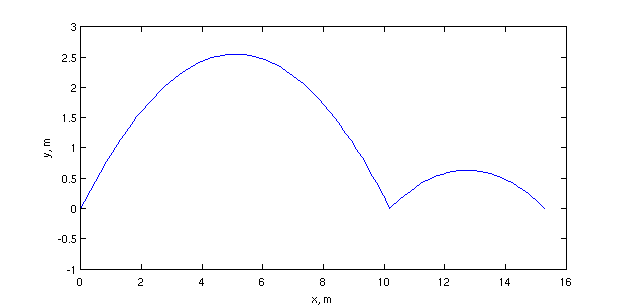
\includegraphics[width=0.9\textwidth]{ball.png}
\end{figure}
}


\plain{
\scriptsize 
Vadim Yudintsev\\
Computational Mechanics with MATLAB\\
Lecture 3: Numerical methods\\
\vspace{10pt}
LaTeX Beamer theme METROPOLIS\\
by Matthias Vogelgesang\\
\href{https://github.com/matze/mtheme}{https://github.com/matze/mtheme}
}
  
  
\end{document}
